\chapter{Cyclone V SoC-FPGA}\label{cap:soc}

% Definição simples de SoC, dois ou três parágrafos e uma imagem
%================================
SoC é um acrônimo de \textit{System-on-a-Chip} ou apenas \textit{System on Chip}, o qual é um sistema computacional inteiro contido em apenas um circuito integrado. Sendo assim, um SoC pode combinar diferentes elementos, em diferentes configurações, para formar um sistema completo.  Portanto um SoC não se restringe à apenas um processador: além da CPU,  ele integra memória, periféricos de controle (por exemplo, barramento de comunicação USB), unidade de processamento gráfico e outros periféricos específicos para uma determinada aplicação.  

Para \citeonline{MichelSoC}, um system-on-chip é uma arquitetura que estabelece uma montagem de processadores, memórias, e interconexões feitos sobre medida para uma determinada aplicação. A figura~\ref{fig:socbasic} ilustra um SoC com alguns elementos básicos, que pode incluir múltiplos processadores  de diferentes arquiteturas, interconectados com uma ou mais memórias, o que pode oferecer meios de se criar sistemas reconfiguráveis, adicionando maior flexibilidade a um SoC.  Em muitas ocasiões um SoC pode ser equipado com componentes analógicos, como conversores analógico-digitais.


\begin{figure}[ht]
	\caption{Esquema SoC básico}
	\begin{center}
		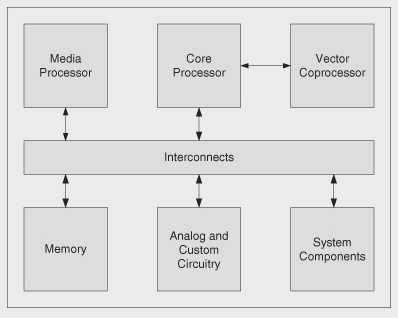
\includegraphics[scale=0.68]{imagens/basicsoc.png}\\
		{\small \textbf{Fonte:} \citeonline{MichelSoC}}
    \end{center}\label{fig:socbasic}
\end{figure}

% Descrição Cyclone V pincipais característica, famílias, imagem 
%================================

Dentre os dispositivos classificados como SoC, a Intel fornece uma linha de produtos classificados como SoC-FPGA, os quais se caracterizam por possuir um rede de FPGA integrados a um Processador ARM\@. Uma família de produtos que possuem essa característica é a Cyclone V SoC-FPGA\@. Estes componentes são constituídos por um \textit{Hardware Processor System} (HPS) que possui processadores ARM Cortex-A9 de um ou dois núcleos e um FPGA\@. A Figura~\ref{fig:socfpga} oferece uma visão global da integração entre os dois componetes principais do SoC-FPGA da família Cyclone V. 

\begin{figure}[ht]
	\caption{Diagrama de blocos simplificado Cyclone V}
	\begin{center}
		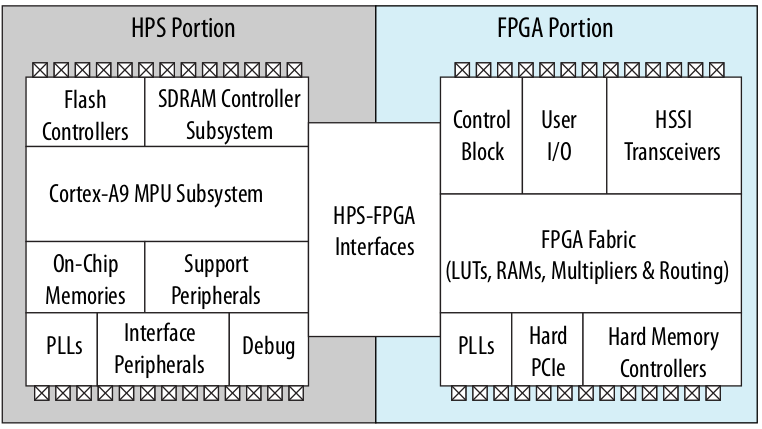
\includegraphics[scale=0.46]{imagens/socfpga.png}\\
		{\small \textbf{Fonte:} \citeonline{alteraCV}}
    \end{center}\label{fig:socfpga}
\end{figure}

Lançada iniciante pela Altera que foi adquirida em 2015 pela Intel~\cite{intelbuyaltera}, a família Cyclone V SoC-FPGA alia o poder de processamento do processador Cortex-A9 à versatilidade e flexibilidade do FPGA, o que faz desta linha de componentes possuir um alto poder de processamento aliado a um baixo consumo. Os caminhos de interconexão entre o HPS e o FPGA do Cyclone V proporciona altas taxas de transferência, o que seria inviável em sistemas com dois chips. Esta estratégia de integração em um único circuito integrado oferece~\cite{CycloneV}:

\begin{itemize}
    \item Largura de banda de pico de mais de 100 Gbps;
    \item Coerência de dados integrada;
    \item Significativa economia de energia do sistema, eliminando caminhos de E/S externos entre o processador e o FPGA\@.
\end{itemize}

Este nível de integração entre os dois componentes que formam o SoC FPGA provê uma solução com baixa potência dissipada, aliado a um reduzido custo e  espaço da placa necessária para a montagem do sistema. Ou seja, o uso dos SoC-FPGA, com processador ARM combinado com FPGA, interligados através de um \textit{backbone} de alta largura de banda e baixa potência, disponíveis nos produtos da linha da família Cyclone V da Intel, possibilita o desenvolvimento de aplicações com excelente desempenho, alta flexibilidade, além de baixo custo e baixo consumo de energia. 

\section{ARM Cortex-A9}
O processador Cortex A9 é uma linha de processadores ARM otimizados para alcançarem maior desempenho aliado a um baixo consumo. Esta linha de processadores ARM é uma das mais utilizadas, nas mais diversas aplicações. O Cortex A9 possui uma estrutura interna configurável, o que oferece flexibilidade ideal para o desenvolvimento de um novo SoC.  Na Tabela~\ref{tab:cortexA9config} são listadas algumas das configurações básicas do processador Cortex A9.

\begin{table}[ht]
    \caption{Confi básicas do ARM Cortex A9 }
    \begin{center}    
        \begin{tabular}{ll}
        \hline \hline
        Arquitetura                     & Armv7-A                                     \\ \hline \hline
        Multicore                       & 1-4 cores                                   \\ \hline \hline
        \multirow{7}{*}{Suporte ISA}    & Armv7-A                                     \\ \cline{2-2} 
                                        & Thumb-2 ou Thumb                            \\ \cline{2-2}
                                        & Tecnologia de segurança TrustZone               \\ \cline{2-2}
                                        & Jazelle DBX e Tecnologia RCT            \\ \cline{2-2}
                                        & Extensão DSP                               \\ \cline{2-2}
                                        & Neon (Opcional)                             \\ \cline{2-2}
                                        & Ponto Flutuante (Opcional)                   \\ \hline \hline
        Unidade de Gerenciamento de Memória (MMU)    & Armv7 MMU                \\ \hline \hline
        Depuração                  & CoreSight                                   \\ \hline \hline
        \multirow{4}{*}{Caracteristicas}& Dual-issue, partially out-of-order pipeline \\ \cline{2-2}
                                        & \begin{tabular}[c]{@{}l@{}}Arquitetura do sistema flexível com
                                            \\caches configuráveis\end{tabular}       \\ \cline{2-2}
                                        & Sistema de coerência com ACP port               \\ \cline{2-2}
                                        & \begin{tabular}[c]{@{}l@{}}Desempenho 50\% maior do que  
                                            \\ o processador Cortex-A8  configurado 
                                            \\ como \textit{single-core}\end{tabular}          \\ \hline\hline
        \end{tabular}
        \\{\small \textbf{Fonte:} \citeonline{armCortexA9}}
    \end{center}\label{tab:cortexA9config}
\end{table}

\subsection{Cortex-A9 MPCore Processor}
O Cortex-A9 MPCore processor é formado por três partes. Estas partes são componentes configuráveis que proporcionam a flexibilidade necessária para implementação de sistemas dedicados sob medida para determinada aplicação. Os componentes do Cortex-A9 MPCore são~\cite{mpcore}:

\begin{itemize}
    \item De um a quatro processadores Cortex-A9, que podem ser agrupados em um cluster, e um \textit{Snoop Control Unit} (SCU) que pode ser usado para assegurar a coerência do cluster;

    \item Um conjunto de periféricos de memória mapeada, incluindo timer global, watchdog e timer privativo para cada processador contido no cluster; e
    
    \item Um controlador de interrupção integrado que é uma implementação do Generic Interrupt Controller. 
\end{itemize}

É possível implementar apenas um processador no cluster do Cortex-A9 MPCore, para isso, o processador deve ser implementado com suas próprias configurações de hardware. Mesmo contendo apenas um processador um SCU ainda estaré disponível, bem como ACP como um opcional. A Figura~\ref{fig:mpcore} apresenta um diagrama que representa o Cortex-A9 MPCore processor.

\begin{figure}[ht]
	\caption{Cortex-A9 MPCore Processor}
	\begin{center}
		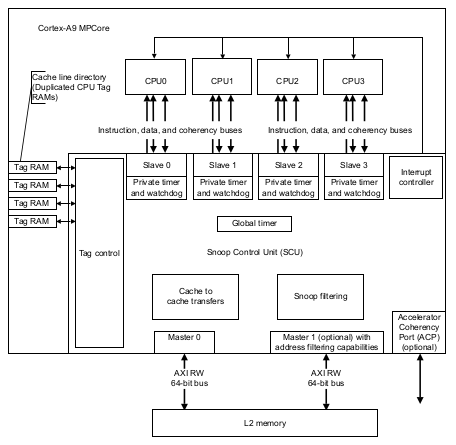
\includegraphics[scale=0.7]{imagens/mpcoreA9.png}\\
		{\small \textbf{Fonte:} \citeonline{mpcore}}
    \end{center}\label{fig:mpcore}
\end{figure}

% \subsection{Protocolo AMBA 3}
% \subsection{Generic Interrupt Control - GIC}

\section{Field-Programmable Gate Array - FPGA}
\textit{Field-Programmable Gate Arrays}, ou simplesmente FPGA, são dispositivos semicondutores construídos através de uma matriz de blocos lógicos configuráveis, os CLBs~\cite{FPGAXilinx}. Estes blocos lógicos são interconectados a partir de conexões programáveis, o que permite ao projetista conectar esses blocos em configurações capazes de executar qualquer tarefa, desde simples portas lógicas até complexas funções.

Os FPGAs foram batizados como dispositivos programáveis em campo devido a capacidade de terem seu hardware reconfigurado pelo usuário, para executar uma função desejada, mesmo após seu processo de fabricação. Esta característica permite que atualizações e soluções de possíveis erros de projetos sejam executadas em campo. São estas características que diferem os FPGAs dos circuitos integrados de aplicação específicas, também conhecidos como ASICs - \textit{Application Specific Integrated Circuits}, que como o nome já sugere, são circuitos desenvolvidos e fabricados para desempenharem apenas uma tarefa específica.

Extremamente versáteis, os FPGAs permitem que desenvolvedores testem inúmeras aplicações mesmo depois que o próprio FPGA e todo o hardware auxiliar já estarem montados em suas placas. Se por algum motivo uma nova configuração for necessária, novos arquivos de configuração podem ser transferidos para o FPGA, fornecendo ao dispositivo novas funcionalidades ou mesmo correção de defeitos. FPGAs são poderosas ferramentas de prototipagem devido à sua flexibilidade, mesmo depois do hardware já estar montado. Aplicações comerciais normalmente usam FPGAs em produtos finais quando a necessidade de computação paralela e requerimentos dinâmicos são um requisito do sistema~\cite{FPGAarm}.



\section{Hardware Processos System}
Como foi mencionado no início deste capítulo, a família de dispositivos Cyclone V system-on-a-chip (SoC) é formada por duas partições, uma malha de FPGA e um processador Arm Cortex-A9, que pode estar organizado em dois ou apenas um núcleo. Esta última partição é chamada de \textit{Hard Processor System} (HPS). 

Os principais módulos do HPS são:

\begin{itemize}
    \item Microprocessador Unit - MPU, subsistema com um ou dois ARM Cortex-A9 (MPCore Processor)
    \item Controladores de memória Flash;
    \item Controladores de SDRAM;
    \item Sistema de interconexão;
    \item On-chip memória; e
    \item Phase-locked loops (PLLs).
\end{itemize}


\subsection{FPGA Manager}
O \textit{FPGA Manager} é o bloco do \textit{Hard Processor System} responsável por gerenciar e monitorar a malha de FPGA presente no SoC. Através do \textit{FPGA Manager} o projetista é capaz de configurar o FPGA, monitora seu estado, além de enviar dados entre o HPS e o FPGA\@. 

\begin{figure}[ht]
	\caption{Diagrama de blocos FPGA Manager }
	\begin{center}
		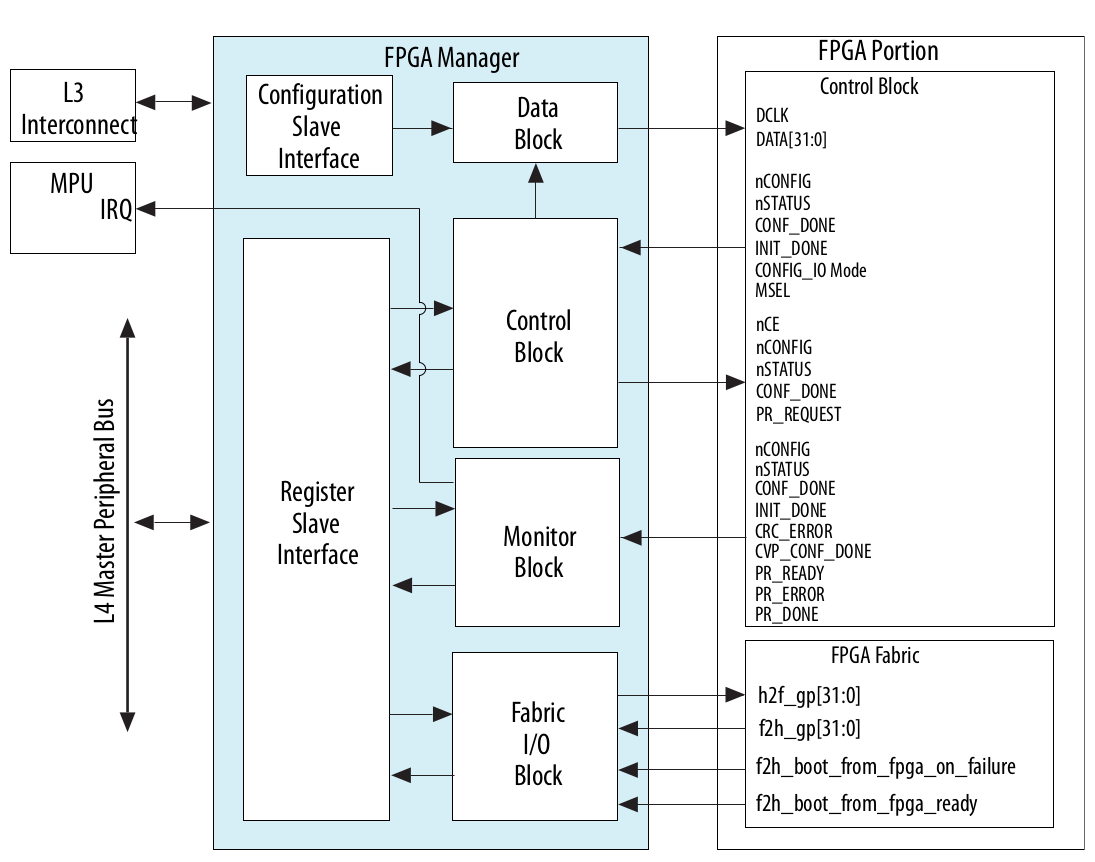
\includegraphics[scale=0.3]{imagens/fpgamanager.png}\\
		{\small \textbf{Fonte:} \citeonline{alteraCV}}
    \end{center}\label{fig:fpgamanager}
\end{figure}

O \textit{FPGA manager} possui as seguintes funcionalidades:

\begin{itemize}
    \item Capacidade de realizar configuração parcial ou completa de toda a malha do FPGA\@;
    \item Enviar 32 sinais de uso geral  do HPS para o FPGA\@;
    \item Receber 32 sinais de uso geral do FPGA para o HPS\@;
    \item Monitorar o status de configuração e potência do FPGA\@;
    \item Gerar interrupções para o HPS a partir das mudanças de status do FPGA\@; e
    \item Capacidade de resetar o FPGA\@.
\end{itemize}

Na Figura~\ref{fig:fpgamanager} podemos ver os principais blocos que formam o sistema do \textit{FPGA Manager}, O \textit{Registrer Slave Interface} se conecta ao L4 \textit{Master Peripheral Bus} fornecendo acesso ao registro de \textit{status} da malha do FPGA\@. Já o \textit{Configuration slave interface} se conecta ao \textit{L3 interconnect} da MPU fornecendo um caminho para que o FPGA possa ser reconfigurado a partir do HPS\@.

Do lado da malha do FPGA, o \textit{FPGA Manager} possui dois blocos, o \textit{fabric I/O} e o \textit{monitor}. No bloco \textit{fabric I/O} os registradores \textit{General-purpose input register} (gpi), \textit{General-purpose output register} (gpo) e \textit{Boot handshaking input register} (misci) possibilitam a comunicação entre o HPS e a malha do FPGA\@. Estes registradores só são acessíveis quando o FPGA está no modo usuário, modo ao qual o FPGA pode ser reconfigurado a partir do HPS\@. O bloco \textit{monitor}, como pode ser deduzido pelo seu nome, fornece uma interface para o monitoramento da malha do FPGA, este bloco monitora sinais relacionados com a configuração do FPGA 


\subsection{HPS-FPGA Bridge}
O HPS pode se comunicar com a malha do FPGA a partir de barramentos de alto desempenho, que podem alcançar larguras de banda superiores a 100Gbps. Estes barramentos, chamados de HPS-FPGA Bridge, usam o protocolo \textit{Advanced Microcontroller Bus Architecture} (AMBA) \textit{Advanced eXtensible Interface} (AXI), o qual foi desenvolvido pela própria ARM, constituindo-se num padrão de conexão dos blocos internos dos dispositivos ARM\@. A Figura~\ref{fig:hpsfpgabridge} exibe o diagrama de blocos das conexões de todas a pontes presentes do Cyclone V.

\begin{figure}[ht]
	\caption{Diagrama de blocos HPS-FPGA Bridge}
	\begin{center}
		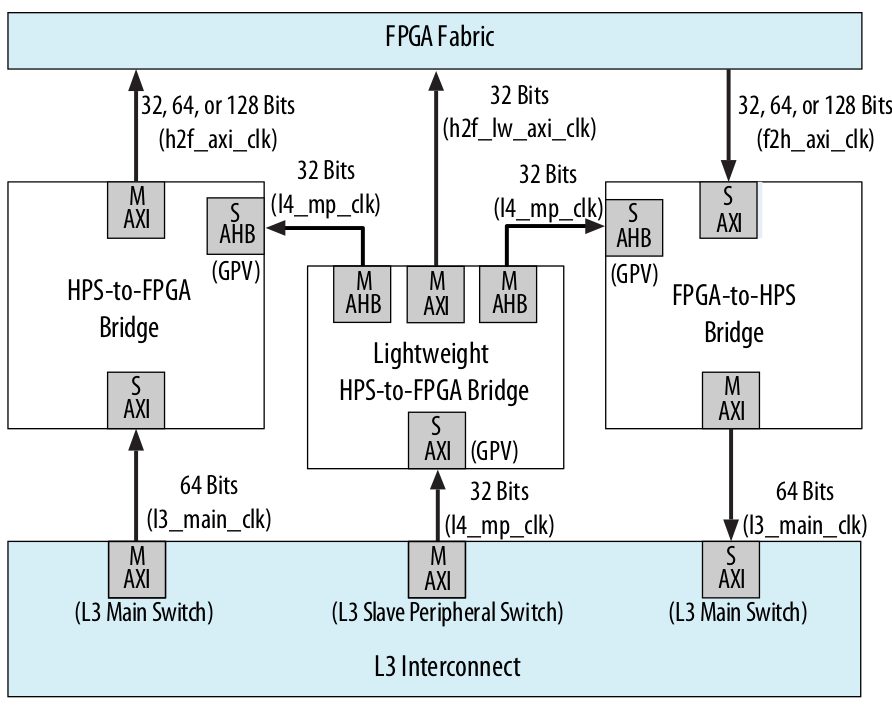
\includegraphics[scale=0.35]{imagens/hps-fpga_bridge.png}\\
		{\small \textbf{Fonte:} \citeonline{alteraCV}}
    \end{center}\label{fig:hpsfpgabridge}
\end{figure}

O HPS possui três pontes, são elas: \textit{FPGA-to-HPS Bridge}, \textit{HPS-to-FPGA Bridge} e a \textit{Lightweight HPS-to-FPGA Bridge}. Estas pontes permitem a comunicação entre o HPS e o FPGA e vice-versa, ou seja, quando o projetista incorpora periféricos ao seu projeto no FPGA, o processador pode acessar esses periféricos através de um barramento de alta velocidade. Como foi dito, essa comunicação também funciona no sentido inverso, do FPGA para o HPS, significando que um componente implementado no FPGA pode acessar regiões de memória e/ou periféricos do HPS\@.


\subsection{Cortex-A9 Microprocessor Unit Subsystem}
Os SoCs da família Cyclone V incluem um \textit{Hard Processor System} formado por um Arm Cortex-A9 MPCore, com processador de uso geral de 32 bits com um ou dois núcleos, um L2 cache, um \textit{Accelerator Coherency Port} (ACP) e módulo de depuração. Tanto o processador como outros módulos no HPS podem acessar blocos lógicos instaciados no FPGA através do \textit{HPS-to-FPGA bridge}. Na Figura~\ref{fig:mpusubsystem} é apresentado um diagrama de blocos simplificado do MPU\@.

\begin{figure}[ht]
	\caption{Cortex-A9 Microprocessor Unit Subsystem com bloco do sistema de interconexão}
	\begin{center}
		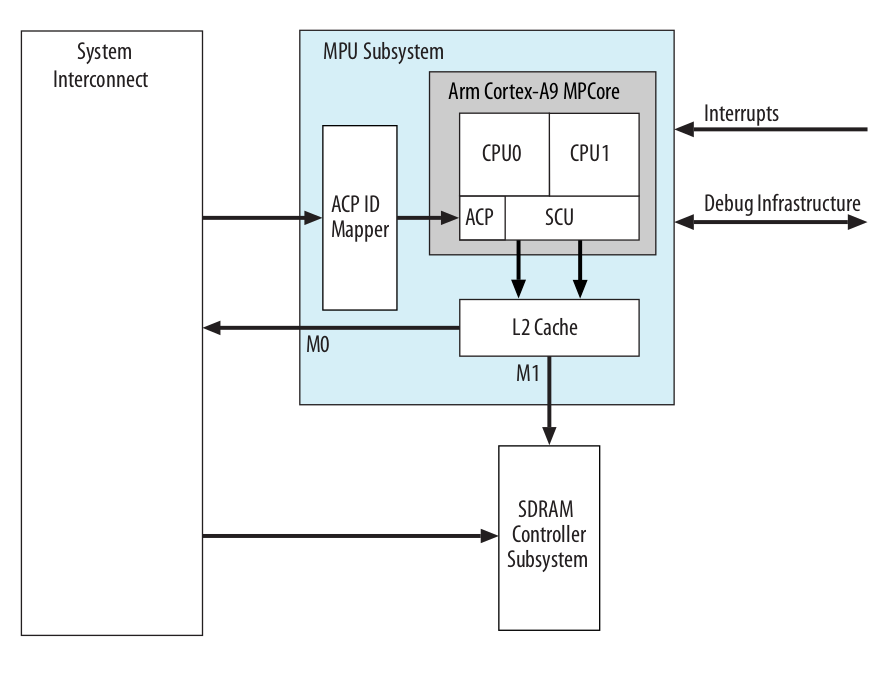
\includegraphics[scale=0.37]{imagens/mpusubsystem.png}\\
		{\small \textbf{Fonte:} \citeonline{alteraCV}}
    \end{center}\label{fig:mpusubsystem}
\end{figure}


\section{Kit de desenvolvimento DE10-nano}

Para o desenvolvimento deste trabalho foi escolhido o kit de desenvolvimento DE10-Nano da Terasic. Construído com base no SoC Cyclone® V SE 5CSEBA6U23I7 integrado com um processador ARM Cortex-A9 dual-core. O kit disponibiliza toda a estrutura básica de hardware necessário para que usuários possam aproveitar todo o poder do hardware reconfigurável oferecido pelo FPGA, combinado com um processador de alto desempenho. Além do SoC Intel, a placa DE10-Nano (Figura~\ref{fig:de10-nano}) oferece excelentes recursos, como memória DDR3 de alta velocidade, conversor analógico-digital, interface USB e interface de rede gigabit ethernet, os quais dão ao kit grande flexibilidade no desenvolvimento de novas aplicações. 

\begin{figure}[ht]
	\caption{Kit de desenvolvimento DE10-Nano}
	\begin{center}
		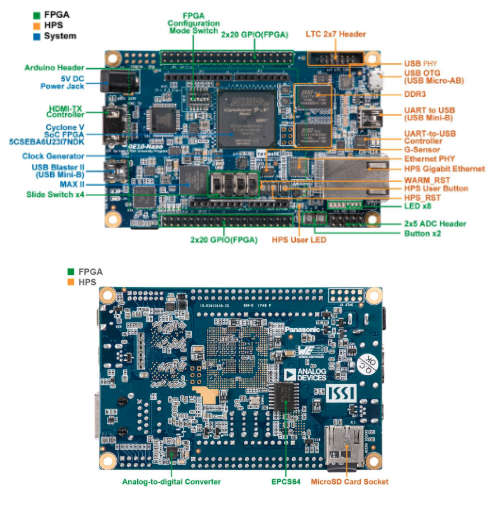
\includegraphics[scale=0.65]{imagens/de10nano.png}\\
		{\small \textbf{Fonte:}\cite{DE10nano}}
    \end{center}\label{fig:de10-nano}
\end{figure}
